\newpage
\chapter{Observables overview}
\mbox{}\vspace{-\baselineskip}
\label{Chapter_observables}

The observables described in this Chapter are considered to be sensitive to color transparency (CT) effects and therefore are suggested to be measured to study the process of $p$ knock-out from a deuteron in the NICA SPD experiment. See Section~\ref{Chap:kin} for the description of the process kinematics and the related kinematic variables.

One observable sensitive to CT effects is nuclear transparency ($T$), which is defined as the cross section of a particular process off a nucleus ($\sigma_{exp}$) divided over the cross section of the same process calculated in the impulse approximation (IA). 
\begin{equation}
T = \frac{\sigma_{\textrm{exp}}}{\sigma_{\textrm{IA}}}.\label{eq:nucl_transp}
\end{equation}

Full color transparency regime, which is expected at ultrarelativistic energies (beam energies $\geq$ 100~GeV), will correspond to $T = 1$. This situation would result in the formation of the point-like configurations (PLCs) that would propagate through the nucleus without soft rescattering in the initial or final state (absence of ISI/FSI). At intermediate energies available at the NICA collider ($\sim$ 10~GeV), full CT regime will not be accessible because on this energy scale, the PLCs expand to the ``normal" hadron size. However, some indications of the transition into the CT regime can still be observed and measured.



In Eq.~\eqref{eq:nucl_transp}, $\sigma_{\textrm{IA}}$ in the denominator is estimated theoretically and therefore, calculation of the nuclear transparency ($T$) boils down to experimental cross section measurements. The cross section of the process $pd\rightarrow ppn$ depends on four kinematic variables, which are described in Section~\ref{Chap:kin}.

The dependence of the nuclear transparency ($T$) on the transverse momentum of the spectator neutron ($p_{st}$) is very informative. Figure~\ref{fig:T_larionov} (left) shows theoretical predictions for this dependence for the process $pd\rightarrow ppn$, and possible contributions from the CT effects are shown by the gray band. The region of small $p_{st}$ in Fig.~\ref{fig:T_larionov} (left) corresponds to the dominance of nuclear absorption effects, which leads to $T < 1$. For $p_{st} > 0.2$~GeV/c, rescattering of the final particles off the spectator comes into play, resulting in growing $T$ and eventually in $T > 1$. See more details in Ref.~\cite{Larionov:2025equ}.


\newpage
Other observables sensitive to the CT effects are the deuteron tensor analyzing powers (spin asymmetries), whose diagonal components are defined by Eq.~\eqref{eq:tensor_power}.
\begin{equation}
A_{\alpha\alpha} = \frac{\sigma_{\alpha}(+1) + \sigma_{\alpha}(-1) - 2\sigma_{\alpha}(0)}{\sigma_{\alpha}(+1) + \sigma_{\alpha}(-1) + \sigma_{\alpha}(0)},\label{eq:tensor_power}
\end{equation}
where $\sigma_{\alpha}(\lambda_{d})$ is the differential cross section for the fixed projection $\lambda_{d}$ of the deuteron spin on the $\alpha$-axis ($\alpha = x,~y,~z $). Note that $A_{xx}+A_{yy}+A_{zz} = 0$ is a universal property of the spin-quadrupol operator. 

In general, off-diagonal tensor analyzing powers (such as $A_{xy}$ or $A_{xz}$) are sensitive to color transparency effects, too, but they are unlikely to be measured because such measurements would require specific (non-standard) deuteron polarization settings that would hardly be experimentally available at NICA.



\begin{figure}[htp]
\begin{center}
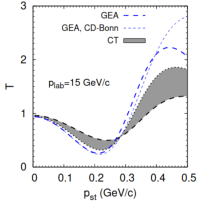
\includegraphics[width=7.4cm]{pictures/T.pdf}
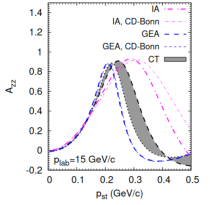
\includegraphics[width=7.4cm]{pictures/Azz.pdf}
\caption{\small  Theoretical calculations for the nuclear transparency $T$ (left) and tensor analyzing power $A_{zz}$ (right) for the process $pd\rightarrow ppn$. Both observables are plotted as functions of the transverse momentum of the spectator neutron ($p_{st}$). The calculations are performed in the framework of the generalized eikonal approximation (GEA) supplemented by the quantum diffusion model of CT~\cite{Frankfurt:1996uz,PhysRevC.107.014605,Larionov:2025equ,Farrar:1988me}. With the color transparency effects included, the presented variables are expected to be within the gray bands, respectively. Both figures are taken from Ref.~\cite{Larionov:2025equ}, where more details on the performed calculations can be found.} \label{fig:T_larionov}
\end{center}
\end{figure}


Figure~\ref{fig:T_larionov} (right) shows theoretical predictions for the dependence of the $A_{zz}$ asymmetry on the transverse momentum of the spectator neutron ($p_{st}$) for the process $pd\rightarrow ppn$. As seen from the plot, CT contributions (shown by the gray band) affect the width of the distribution and the position of its maximum and are the most prominent at $p_{st} = 0.3$~GeV/c. See more details in Ref.~\cite{Larionov:2025equ}.

Theoretical calculations presented in Fig.~\ref{fig:T_larionov} were performed in the framework of the generalized eikonal approximation (GEA) supplemented by the quantum diffusion model of CT~\cite{Frankfurt:1996uz,PhysRevC.107.014605,Larionov:2025equ,Farrar:1988me}. Both plots in Fig.~\ref{fig:T_larionov} are taken from Ref.~\cite{Larionov:2025equ}, where more details on the performed calculations can be found. The gray bands in the presented plots correspond to different values of the parameter $\Delta M$ (which is the only free parameter of the model). This parameter is related to the coherence length, which describes the scale on which the PLCs expand to the ``normal" hadron size. A brief description of the model formalism is given in Appendix~\ref{app_formalism}.

Dependences of the nuclear transparency ($T$) and the tensor analyzing powers ($A_{\alpha\alpha}$) on the azimuthal angle between the scattered proton and the spectator neutron are also of interest, and therefore, suggested to be measured, too (if experimental statistics permits).

Additionally, vector analyzing powers $A_{\alpha}$ ($\alpha$ = $x$,~$y$,~$z$) and their azimuthal dependences are also sensitive to color transparency effects (especially, $A_{y}$). However, these observables are small and hence are not expected to be easily measured. It is also remarkable that for the impulse approximation (which would correspond to the full color transparency regime accessible at ultrarelativistic energies), vector analyzing powers $A_{\alpha}$ are identically equal to zero.


Thus, to investigate color transparency effects for the process of $p$ knock-out from a deuteron in the upcoming SPD experiment with the NICA collider, we suggest to measure the nuclear transparency $T$ (which is equivalent to cross section measurements) and the tensor analyzing powers $A_{\alpha\alpha}$ (and possibly, vector analyzing powers $A_{\alpha}$) as functions of the transverse momentum of the spectator neutron ($p_{st}$) and (if statistics permits) the azimuthal angle between the scattered proton and the spectator neutron. The measured observables will then be theoretically analyzed using the approach from Refs.~\cite{Frankfurt:1996uz,PhysRevC.107.014605,Larionov:2025equ,Farrar:1988me} in order to make a conclusion about possible contributions from the CT effects.



